\documentclass[preprint]{elsarticle}

\usepackage{lineno,hyperref}
\modulolinenumbers[5]

\journal{To be determined}
\usepackage{graphicx}
\usepackage{epstopdf}
\usepackage{mathptmx}
\usepackage{amsmath}
\usepackage{amssymb}
\usepackage[linesnumbered]{algorithm2e}
\usepackage{algcompatible}
\usepackage{enumerate}
\usepackage[english]{babel}
\usepackage{multirow}
\usepackage{tabularx}  % for 'tabularx' environment and 'X' column type
\usepackage{ragged2e}  % for '\RaggedRight' macro (allows hyphenation)

%appendix name fix
\usepackage[english]{babel}

%Pretty tables
\usepackage{booktabs}
\setlength\heavyrulewidth{0.2ex}
\setlength\lightrulewidth{0.15ex}
\setlength\cmidrulewidth{0.15ex}

\usepackage{caption}
\usepackage[utf8]{inputenc}
\usepackage{subcaption}

%for drawing over the notation table
\usepackage{tikz}

%set double spacing
\usepackage{setspace}

%Allow more figures per page
\renewcommand{\floatpagefraction}{.999}


%%%%%%%%%%%% FIX SECTIONS LATEXDIFF %%%%%%%%%%%%%%%%%%%%%
\usepackage{xcolor}
\DeclareRobustCommand{\hsout}[1]{\texorpdfstring{\sout{#1}}{#1}}
\DeclareRobustCommand{\hwave}[1]{\texorpdfstring{\uwave{#1}}{#1}}
\RequirePackage[normalem]{ulem}% DIF PREAMBLE
\RequirePackage{color}\definecolor{DELETIONS}{rgb}{1.0,0.0,0.0}
\RequirePackage{color}\definecolor{ADDITIONS}{rgb}{0.0,0.6,0.0}
\providecommand{\DIFadd}[1]{{\protect\textcolor{ADDITIONS}{\hwave{#1}}}}% DIF PREAMBLE
\providecommand{\DIFdel}[1]{{\protect\textcolor{DELETIONS}{\hsout{#1}}}}% DIF PREAMBLE
%\providecommand{\DIFdel}[1]{{\protect}}% DIF PREAMBLE

%%%%%%%%%%%%%%%%%%%%%%%%%%%%%%%%%%%%%%%%%%%%%%%%%%%%%%%%%%%%%%%

\usepackage{verbatim}

\begin{document}

\title{Improving recommendation of useful pieces of information for users to better understand current context}

\begin{spacing}{2}

\begin{frontmatter}

\author[addressjorge,addressjie]{Jorge Castro\corref{mycorrespondingauthor}}
\ead{jcastro@decsai.ugr.es}

\author[addressjie]{-Jie Lu}
\ead{jie.lu@uts.edu.au}

\author[addressjie]{-Guangquan Zhang}
\ead{guangquan.zhang@uts.edu.au}

\author[addressluis]{Luis Mart\'inez}
\cortext[mycorrespondingauthor]{Corresponding author}
\ead{martin@ujaen.es}

\address[addressjorge]{Department of Computer Science and Artificial Intelligence, University of Granada, Granada (Spain)}
\address[addressjie]{School of Software, University of Technology Sydney, Sydney (Australia)}
\address[addressluis]{Computer Science Department, University of Ja\'en, Ja\'en (Spain)}

\begin{abstract}

Recommender systems (GRSs) filter relevant items to users in overloaded search spaces using information about their preferences. In this scenario, there are succesful RSs for several domains including recommendation of news and QA, among others. The traditional recommendation scheme consists of analysing the terms used in the item to generate an item profile and a user profile that later is used to recommend items that match user profiles. This basic scheme can be further improved considering that context influences user preferences. Some examples of contexts are the device where the recommendations are shown, companion of the target user or trends in current interest according to what others talk about. In the latter case, there have been . This paper focuses on the context extracted from the latter scenario, in which a feed of status updates of a well-known social network is used. When the information is extracted in such a way, there are several key aspects in the context integration with the user profile, such as context cleaning, aggregation and weighting. This paper explores such aspects and proposes a recommender system that integrates context to improve QA recommendation with context information. A case study will evaluate the results on several datasets, showing that the context integration benefits recommendation.

\begin{keyword}
   \texttt{recommender systems} \sep \texttt{context-aware recommendation} \sep \texttt{user profile contextualisation}
\end{keyword}
\end{abstract}

\end{frontmatter}

\section{Introduction}\label{sec:introduction}

\section{Proposal}

The proposal is composed of several parts:
11
\begin{enumerate}
	\item Extract information of the QA domain.
	\begin{itemize}
		\item TfIdf
		\item LSA over TfIdf
	\end{itemize}
	\item Building user preference profile: Aggregate 
	\item Context profile building
	\item Contextualization of user profiles
	\item Prediction
\end{enumerate}


\section{Extract information of the QA domain.}

In the QA dataset there is textual information of the question and its related answers. In this proposal we treat all the i

\subsection{TfIdf}

In this proposal we consider posts as the document, and the words used in their text as the terms. The terms are stemmed using the Porter Stemmer algorithm \citep{Porter1980}. Once stemmed, their term frequency is computed using the raw count of appearance on the document:
\begin{equation}
	profile_{d} = \{tf_{t,d}~~~~s.t.~~~~ t \in d \} ~~~~,  ~~~~~~
	tf_{t,d} = f_{t,d}
\end{equation}

Once the term frequency is computed for all terms in all documents, the inverse document frequency is calculated for each term.

\begin{equation}
	idf_t = - \log( N / n_t )
\end{equation}

Finally, the values of the profiles are weighted with the $idf_t$ of each term:
\begin{equation}
	profile_d = \{w_{t,d} ~~~~s.t. ~~~~t\in d\} ~~~~,  ~~~~~~
	w_{t,d} = tf_{t,d}*idf_t
\end{equation}

\subsection{LSA over TfIdf}

Once the tf-idf profiles are built, LSA is performed to reduce the dimensionality of the matrix. LSA is proven to be effective through the description of both document and words in a reduced number of features, while reducing the negative impact of synonyms in the text \cite{}. Therefore, the aim of this step is to decompose the word-document in: word-features matrix ($U$), singular value vector ($s$), and document-features matrix ($V$):

\begin{equation}
	TFIDF_{(|D|\times|T|)} = U_{(|D|\times k)} * s_{(k)} * V'_{(k \times |W|)}
\end{equation}

The proposal performs an approximated factorisation of the TF-IDF matrix using singular value decomposition, which allows to reduce the dimensionality of the original matrix keeping the $k$ most relevant singular values of the original matrix.

Hence, we obtain the profile of both terms and documents in the reduced space:
\begin{equation}
	profile_d = \{ U_{t,1},\dots, U_{t,k}\}
\end{equation}

\begin{equation}
	profile_t = \{ V_{t,1},\dots, V_{t,k}\}
\end{equation}

\section{Building user preference profile: Aggregate words' profiles}

At this point the proposal has built a model to describe documents and words. In order to provide personalised recommendation to users, it is needed to build user profiles in the same space. The information the system holds about users is a unary matrix that states whether the user has expressed interest in the document either by creating, commenting, or voting it:

\begin{table}
	\caption{Users' preferences over items, the rating matrix.}
	\label{tab:user-preferences}
	\centerline{\small\baselineskip=13pt
	\begin{tabular}{|c||ccccc|}
		\hline
         &     $i_1$     & $\dots$  &     $i_k$     & $\dots$  & $i_n$
		\tabularnewline
		\hline
		\hline
$u_1$    & $r_{u_1,i_1}$ & $\dots$  & $r_{u_1,i_k}$ & $\dots$  & $r_{u_1,i_n}$
		\tabularnewline
$\vdots$ & $\vdots$      & $\ddots$ & $\vdots$      & $\ddots$ & $\vdots$
		\tabularnewline
$u_j$    & $r_{u_j,i_1}$ & $\dots$  & $r_{u_j,i_k}$ & $\dots$  & $r_{u_j,i_n}$
		\tabularnewline
$\vdots$ & $\vdots$      & $\ddots$ & $\vdots$      & $\ddots$ & $\vdots$
		\tabularnewline
$u_m$    & $r_{u_m,i_1}$ & $\dots$  & $r_{u_m,i_k}$ & $\dots$  & $r_{u_m,i_n}$
		\tabularnewline
		\hline
	\end{tabular}}
\end{table}

With this table we can get the set of documents that user $u$ has expressed interest in:
\begin{equation}
	R_{u} = {d ~~~~s.t.~~~~r_{u,d} =1 }
\end{equation}

This way, the user profile is built upon the profiles of the documents that belong to $R_u$:

\begin{equation}
	profile_u = \sum_{d \in R_u} V_d = \{ \sum_{d \in R_u} V_{d,1}, \dots, \sum_{d \in R_u} V_{d,k}\}
\end{equation}

This user profile describes the user preferences in terms of the singular values.

\section{Context profile building}

In parallel with the building of the user profile, it is needed to build the context profile. In this proposal we assume that the source of the context is a microblogging system that delivers status updates by users. To narrow down the status updates that the system receives in order to focus in an aspect of the context. Therefore, there is a set of terms that must appear in the status updates:

\begin{equation}
	\forall d \in Context \exists t \in d \wedge t\in T_c
\end{equation}

Based on the terms that appear on the context we can build the profile of the context using the feature representation of each term from the QA domain.

\begin{equation}
	profile_{T_c} = \{\sum_{t \in T_c} U_{t,1}, \dots, \sum_{t \in T_c} U_{t,k} \}
\end{equation}

\section{Contextualization of user profiles}

Once we have the user profile and the context profile, it is needed to combine them in order to provide personalised recommendation that are suited to the current context $T_c$:

\begin{equation}
	profile_u^{T_c} = \alpha * profile_u + (1- \alpha )*profile_{T_c}
\end{equation}

\begin{equation}
	profile_u^{T_c} = \{ \alpha * profile_{u,1} + (1- \alpha ) * profile_{T_c,1},\dots, \alpha * profile_{u,1} + ( 1 - \alpha ) * profile_{T_c,k} \}
\end{equation}

\section{Prediction}

Once we have the contextualised user profile, we can produce a prediction of the suitability for a given item regarding the profile:
\begin{equation}
	p_{u,d} = profile_u^{T_c}*s*profile_d
\end{equation}

The recommendation is a list of documents sorted by $p_{u,d}$.

\section{Experiment}

To evaluate the proposal, we performed an experiment that simulates the recommendation of QA items in in various context. The remainder of the section is structured as follows. First, the settings of the experiment are described. The datasets and methods for processing are then detailed. After that, the evaluation measures are commented. Lastly, the results are analysed.

\subsection{Experimental procedure}

In these experiments, a RS based on LSA modelling with contextual information is evaluated (LSAContext). The baseline method to compare with is the LSA method without contextual information. 30 features are considered in LSA and LSAContext models.

In order to do the experiment, the following procedure is performed \cite{Sarwar2001}, with a modification to consider contextual information in the experiment:
\begin{itemize}
	\item Split the dataset in training and test.
	\item Build the model with the training data.
	\item Build the profile of each user. Include contextual information.
	\item Recommend to each user based on their profile and the model.
	\item Evaluate recommendations with the test set.
\end{itemize}

This procedure is repeated 20 times and 5-cross fold validation is used to split the data in training and test sets. Moreover, various contexts are considered, which are detailed in the following section.

\subsection{Datasets}

In the experiment there are two sources of data: The QA domain and the contextual information.

The QA domain used is the StackExchange dataset\footnote{http://data.stackexchange.com/}. This dataset consists of the database dump of each site in the stackexchange ecosystem. Some sites are detailed in Table \ref{tab:stackexchange-dataset-description}, together with their main features.

In this experimental setup, the results are reported per StackExchange site. Therefore, we consider each site as a different dataset. Given that the aim of the system is to provide users with pieces of information that help explain the context and also consider their preferences.

Regarding the contextual dataset, a set of interesting keywords is defined. We have selected the terms \emph{news}, \emph{current} and \emph{situation}. From these seed terms, we extracted a dataset of tweets that contain any of these words from twitter. The stats of the dataset extracted is depicted in Figure \ref{fig:context-dataset-description}.

\begin{figure}[htb]
    \centering
    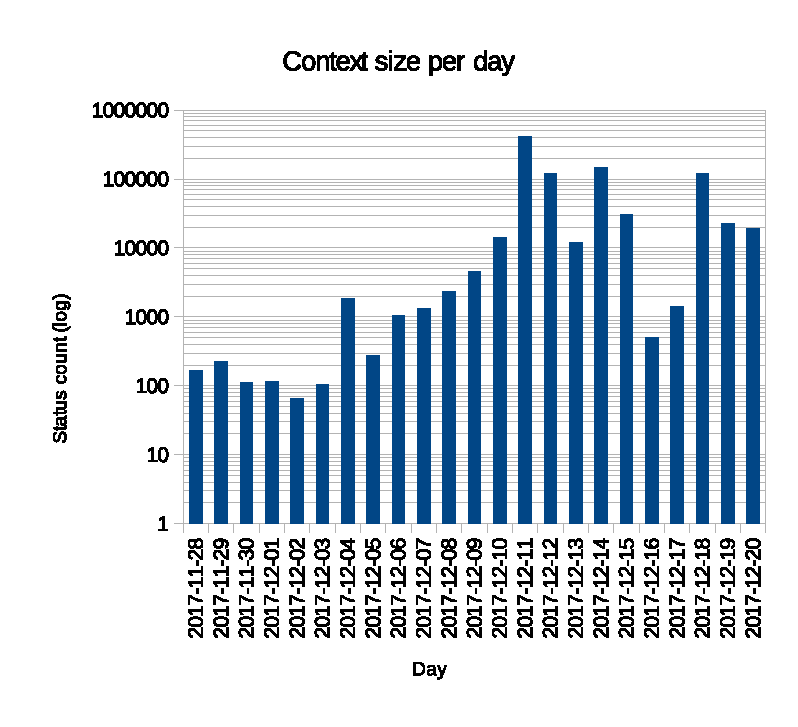
\includegraphics[width=0.5\textwidth]{figures/context-dataset-description.eps}
    \caption{Contextual dataset used in the experiment, where each day has a different status count.}
    \label{fig:context-dataset-description}
\end{figure}

\subsection{Evaluation Measures}

Usually, measures to evaluate the prediction errors in terms of rating deviation are used. However, the methods being compared do not provide a rating prediction, but a value that expresses the suitability of items regarding the user profile. Therefore, the measures that can be used are information retrieval ones, such as precision and recall. Researchers have remarked that, although they are useful, they are not sensible to the sorting of the items that the RSs does \cite{Gunawardana2015}. In order to consider the quality of the sorting, the NDCG is used:

\begin{equation}
	DCG_u = \sum_{k=1}^N\frac{r_{u,recom_{u,k}}}{log_2 (k+1)}
\end{equation}

\noindent where $recom_{u,k} \in I$ is the item recommended to user $u$ in $k$ position.

\begin{equation}
	NDCG = \frac{DCG}{DCG_{perfect}}
\end{equation}

\noindent where $DCG_{perfect}$ is a perfect sorting of the items, i.e., the list of items sorted by their value in the test set.

\subsection{Results}

In this section, the results obtained for the different approaches compared are shown and analysed to evaluate the performance of the proposal.

Table \ref{tab:results-ndcg-3dprinting} shows the results of the compared approaches in the 3dprinting site.


\textbf{\textit{Acknowledgements:}} This research work was partially supported by the Research Project TIN-2015-66524-P, the Spanish FPU fellowship (FPU13/01151), and also the Eureka SD Project (agreement number 2013-2591).

\section*{Bibliography}
\bibliography{rs-bibliography}

\end{spacing}

\end{document}